\documentclass[12pt,a4paper]{scrartcl}
\usepackage[utf8]{inputenc}
\usepackage[english]{babel}
\usepackage{dsfont}
\usepackage{csquotes}
\usepackage{makeidx}
\usepackage[left=3cm,right=2cm,top=2cm,bottom=2cm]{geometry}
\usepackage{setspace}
\usepackage{chngcntr} 
\usepackage{pdfpages}
\usepackage{graphicx}
\graphicspath{ {images/} }
\usepackage{setspace}
\usepackage{caption}
\usepackage{amssymb, amsmath, amsthm}
% \usepackage{mathtools} % Bonus
\usepackage{amsfonts}
\usepackage{amssymb}
\usepackage{graphicx}
\usepackage{float}
\usepackage{lipsum}
\usepackage[]{biblatex}
\addbibresource{references.bib}
\usepackage{color}   %May be necessary if you want to color links
\usepackage{hyperref}
\hypersetup{
    colorlinks=true, %set true if you want colored links
    linktoc=all,     %set to all if you want both sections and subsections linked
    linkcolor=blue,  %choose some color if you want links to stand out
}
\urlstyle{same}



\setlength{\parskip}{10pt} % Abstand zwischen den Absätzen
\setlength{\parindent}{0pt} %Erstzeileneinzug 
\setcounter{secnumdepth}{3}
\setcounter{tocdepth}{4}


\title{Master Thesis}
\date{\today}
\begin{document}
	\begin{titlepage}
		\centering
		University of Bonn
		
		 Master Programme in Economics
		\vspace{1in}
		\vspace{1in}
		
		{\LARGE \bfseries  Random Forest for Classification Problems}
		\vspace{1in}
		
		{\large Submitted by}
		
		{\LARGE Burak Balaban \par
				Arkadiusz Modzelewski\par
				Raphael Redmer\par}
		
		\vspace{1in}
		
			Supervisor: Prof. Dr. Dominik Liebl
			
		\vfill
		
		\begin{flushleft}
			\today
		\end{flushleft}
		
	\end{titlepage}
	

	\tableofcontents
	\thispagestyle{empty}
	\newpage

	%\section*{Abstract}
\thispagestyle{empty}
In this paper, we examine the machine learning algorithm Random Forest
and present the results of its application.
First, we start with an explanation of the Decision Trees.
Then, we proceed to show how it can be improved.
More specifically, these improvements for the Decision Trees contain bagging, boosting and Random Forest.
There, we show that the Random Forest achieves a better prediction accuracy
by introducing randomness in tree ensembling.
This randomness provides us with a decorrelated ensemble of trees and
the increase in the number of uncorrelated trees yields lower error regarding prediction purposes. By using Random Forest, we can assess the importance of every variable
and make conclusions about data.
Moreover, we explain the intuition of Random Forest in detail including mathematical clarification.
Finally, we apply Random Forest on both simulated and real data and compare it with various methods.
In conclusion, this paper aims to introduce the relevant concepts in detail and is essentially a review. 



%As a non-parametric estimation tool, Decision Trees attract attention in the economics literature. 
%Yet, Decision Trees suffer from high variance and, 
%for prediction purposes higher variance seems to be a crucial problem, thus, 
%several improvements were proposed such as bootstrap aggregation, boosting and most importantly random forests. 
%In this project, while the main focus is being on the random forest.
%The elements of statistical learning by \cite{friedman2001elements} \cite{varian2014big} \cite{maimon2005data},
%\cite{louppe2014understanding} and as expected \cite{breiman2001random} are the main literature 
%that will be utilized in this project.

%To explain the concept of random forests in full extent, primarily Decision Trees should be discussed. 
%Exploiting the main idea and struggles with bias-variance trade-off, 
%random forests' importance can be emphasized as a more stable prediction tool \cite{maimon2005data}. 
%Conceptual comparison of random forests with bagging and boosting can deliver a better understanding of 
%its unique features as \cite{lee2019bootstrap} shows in a similar fashion. To get a further understanding, 
%random forests’ estimation process can be mathematical explained \cite{biau2012analysis} and likewise, 
%examining the consistency of estimator and showing the properties can be included \cite{breiman2004consistency}, 
%\cite{denil2014narrowing}. Also, variable importance in the tree growing process is another area that needs to be 
%delved into \cite{ishwaran2007variable} and \cite{louppe2013understanding}.


	\pagenumbering{arabic}

	\section{Introduction}
\label{ch:intro}

Lorem ipsum dolor sit amet, consetetur sadipscing elitr, sed diam nonumy eirmod tempor invidunt ut 
labore et dolore magna aliquyam erat, sed diam voluptua. At vero eos et accusam et justo duo 
dolores et ea rebum. Stet clita kasd gubergren, no sea takimata sanctus est Lorem ipsum dolor sit amet.
Lorem ipsum dolor sit amet, consetetur sadipscing elitr, sed diam nonumy eirmod tempor invidunt ut labore
et dolore magna aliquyam erat, sed diam voluptua. At vero eos et accusam et justo duo dolores et ea rebum.
Stet clita kasd gubergren, no sea takimata sanctus est Lorem ipsum dolor sit amet.

	\section{Decision tree}

%%%%%%%%%%%%%%%%%%%%%%%%%%%%%%%
\subsection{Main idea}
The Decision Tree is a non-parametric supervised learning method used for classification and regression.
It predicts the response with a set of if-then-else decision rules derived from the data.
The deeper the tree, the more complex the decision rules and the closer the model fits the data.
The Decision Tree builds classification or regression models in form of a tree structure.
Each node in the tree further partions the feature space into smaller and smaller subsets, 
while at the same time an associated Decision Tree is incrementally developed.
The final result is a tree with decision nodes and terminal nodes. 
A decision node has two or more branches.
Leaf nodes represent the actual classification or decision. 
The topmost decision node in a tree which corresponds to the best predictor is called the root node.
Decision trees can handle both categorical and numerical data.

An example of such a tree is depicted below in figure \ref{fig:decision_tree_example}.

\begin{figure}[H]
    \captionsetup{format=plain}
    \makebox[\textwidth]{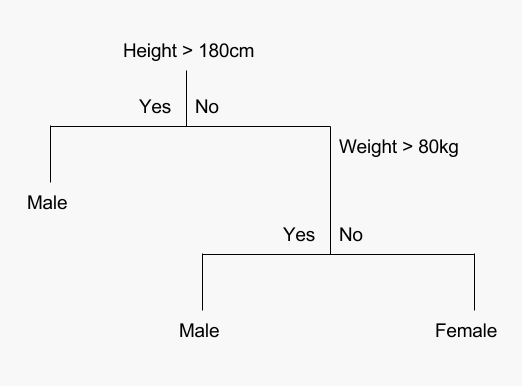
\includegraphics[width=100mm]{decision_tree_example.png}}
    \caption{Given a data set with two features height and weight, and gender as the target variable, 
             this example tree stratisfies the two-dimensional feature space into three distinct subset each 
             represented by the terminal nodes at the bottom.
             The stratification occurs at the two deciding nodes depending either on whether its height is above 180 cm 
             and its weight is above 80kg.
             }
    \label{fig:decision_tree_example}
\end{figure}

%%%%%%%%%%%%%%%%%%%%%%%%%%%%%%%
\subsection{Tree Building Process}
This chapter describes the CART algorithm for tree building as specified in \cite{breiman1984classification}.
The basic idea of tree growing is to choose a split among all the possible splits at each node
such that the resulting child nodes are the “purest”. In this algorithm, only univariate splits are
considered. That is, each split depends on the value of only one predictor variable. All
possible splits consist of possible splits of each predictor.

A tree is grown starting from the root node by repeatedly using the following steps on each
node in the following algorithm:

\begin{algorithm}[H]
    \caption{Binary Splitting \cite{breiman1984classification}}
    \label{alg:binary_splitting}
    \SetAlgoLined
    \begin{itemize}
        \item[(i)] \textbf{Find best split \(s\) for each feature \(X_{m}\):}
        For each feature \(X_{m}\), there exist \(K-1\)-many potiential splits, 
        whereas \(K\) is the number of different values for the respective feature.
        Evaluate each value \(X_{m,i}\) at the current node \(t\) as a 
        candidate split point (for \(x \in X_{m}\), if \(x \leq X_{m,i}=s\),
        then \(x\) goes to left child node \(t_{L}\) else to right child node \(t_{R}\)).
        The best split point is the one that maximize the splitting criterion \(\ \Delta i(s,t) \) the most when the node is split according to it.
        The different splitting criteria will be covered in the next chapter.

        \item[(ii)] \textbf{Find the node’s best split:} Among the best splits for each feature from Step (i) find the 
        one \(s^{*}\), which maximizes the splitting criterion \(\Delta i(s,t)\).

        \item[(iii)] \textbf{Satisfy stopping criterion:} Split the node \(t\) using best node split \(s^{*}\) from Step (ii) 
        and repeat from Step (i) until stopping criterion is satisfied. 
    \end{itemize}
    \end{algorithm}


%%%%%%%%%%%%%%%%%%%%%%%%%%%%%%%
\subsubsection{Splitting criteria}
Since we are only concerned with classification, \(Y\) is categorical. The original CART algorithm uses Gini and Twoing as 
purity measures for the splitting criterion \cite{breiman1984classification}. 
However, implementations of the algorithm such as Python's sklearn package \cite{scikit2011learn} also contain entropy and misclassification rate as measures of impurity.

For a given learning sample \( D = {(x_{1},y_{1}), (x_{2}, y_{2}), ... , (x_{N}, y_{N})} \) 
for a \(C\) class problem, let \(N_{c}\) be the number of instances \( \{x,y\}  \)
belonging to class \(c\).

In node \(t\), let \(N(t)\) be the total number of instances with \( \{x,y\} \in t \) 
and \( N_{c}(t) \) the number of class \(c\) instances in \(t\). 
The proportion of the instances belonging to class \(c\) in the sample \(D\) falling into \(t\) 
equals \( N_{c}(t) / N_{j} \).
The given set of priors \( \pi(c) \) specify the probability that an instance belongs to class \(c\).

At node \(t\), let the probabilities \(p(c,t)\) be estimated by 

\begin{equation}
    p(c,t) = \frac{ \pi(c)N_{c}(t) }{ N_{c} }.
\end{equation}

This represents the probability that an instance will both be in class \(c\) and fall into node \(t\).
Therefore, the estimate for the probability that any instance falls into node \(t\) is defined by

\begin{equation}
    p(t) = \sum_{c \in C} p(c,t),
\end{equation}

The estimate \( p(t) \) for the probability that an instance belongs to class \(c\) given that it falls into node \(t\) is defined by

\begin{equation}
    p(c|t) = \frac{ p(c,t)}{ p(t) } = \frac{ p(c,t) }{ \sum_{c \in C} p(c,t) }.
\end{equation}

Further, it holds that the conditional probability \(p(c|t)\) must satisfy

\begin{equation}
    \sum_{c \in C} p(c|t)  = 1
\end{equation}

Let \(i(t)\) be an impurity measure evaluated at note \(t\). 
Then, the decrease of impurity (i.e. the splitting criterion) is defined as

\begin{equation}
    \Delta i(s,t) = i(t) - p_{L} i(t_{L}) - p_{R} i(t_{R}),
\end{equation}

where \(p_{L}\) and \(p_{R}\) are probabilities of sending a case to the left child node \(t_{L}\) and to the
right child node \(t_{R}\) respectively. 
They are defined as \( p_{L} = p(t_{L}) / p(t) \) and \( p_{R} = p(t_{R}) / p(t) \).

As already stated above, the goal is to maximize \(\Delta i(s,t)\).
In the following, different measures for impurity will be presented.

\textbf{Gini Measure}

The Gini impurity measure is defined as 


\begin{equation}
    i(t) = \sum_{c \in C} p(c|t) (1 - p(c|t)) = 1 - \sum_{c \in C} p_{c}^{2}
\end{equation}

The intuition behind this measure is to assign nodes 
for which its probabilities are more skewed towards a particular group for a higher value.
Conversely, if a node has a more balanced distribution, then \(i(t)\) will turn out to be lower.
For example, in the case of \( |C|=2 \), \(i(t)\) will be maximized by \( p(c|t) = 0.5 \) for \( c \in C \).


\textbf{Information Entropy}

The Entropy measure from information theory is defined as

\begin{equation}
    i(t) = \sum_{c \in C} p(c|t) log(p(c|t)),
\end{equation}

which measures the average rate at which information is produced by a stochastic source of data .
Thus, it can also be used for measuring impurity.


\textbf{Rate of Misclassification}

The rate of misclassification is defined as 

\begin{equation}
    i(t) = 1 - \max_{c \in C} p(c|t) .
\end{equation}

which measures the proportion of instances node \(t\) not belonging to the dominant group in \(t\).


%%%%%%%%%%%%%%%%%%%%%%%%%%%%%%%%%%%%%
\subsubsection{Bias-variance trade-off}
We can measure the the performance of a Decision Tree by assessing its fit to the data. 
The generalization error is a widely used concept for evaluating the fit \cite{breiman2001random}.
In this paper, we use generalization error to compare methods and adjust parameters to improve methods. 
Under certain assumptions, we can decompose the generalization error into three main components:
the Bayes Error, the squared bias ($bias^2$) and the variance. 
We will explain the mathematical aspects of the generalization error in the following chapters. 
For now, we only need to mention the Bayes Error is irreducible and independent of the classifier, 
and there is a trade-off between $bias^2$ and variance. Since Decision Trees suffer from high variance and 
decreasing variance causes $bias^2$ to increase \cite{geman1992neural}, we need methods to bypass this trade-off. 
These methods include Bagging, Boosting and Random Forest 
which exploit mathematical properties to decrease variance without increasing $bias^2$. 
We will explain bagging briefly, exhibit mathematical dynamics of Random Forest and 
use Boosting in the application section.


\subsection{Bagging}
Decision Tree belongs to methods which are sensitive to the specific data on which they are trained \cite{friedman2001elements}. 
In other words, Decision Tree estimates are susceptible to even slight changes in data and 
that stems from having high variance.
%When we change the training data, we can get very different resulting Decision
%Trees, and as a result of that also predictions are different.
Bootstrap Aggregation (bagging) was designed for dealing the high variance problem in Decision Tree estimates.
%Bagging, or, Bootstrap Aggregation is a procedure that can be used for reducing the variance.
L. Breiman introduced bagging for Decision Tree in \cite{breiman1996bagging}.
We start the bagging procedure by conducting bootstrapping.
We draw multiple random subsamples with replacement,
and then we use these datasets as training data for our model.
Therefore, the number of Decision Trees equal that of the subsamples. 
Finaly, we obtain the final estimate of the bagged model by averaging over each estimate of the bootstrapped trees.
As bagging, Random Forest makes use of bootstrapped sampling and employes bagged Decision Trees.
%After introducing bagged Decision Trees, a further improvement to this method was added. 
%The method which contains this improvement over the bagged Decision Tree is as the Random Forest. 
The fundamental difference between bagging and Random Forest is 
injection of randomness included explanatory variables. 
We will go into further details about Random Forest and the additional randomness in the next section.
%This method and mentioned injection of randomness in it will be described in the next section of paper.


	\section{Random Forest}
Decision trees, which we mentioned in the previous section, have been used for a long time. 
Deployment of decision trees is visible in simple situations and also in more complex scientific or real life and industrial affairs.
The recent popularity of decision trees is due to work presented by 
\cite{Breiman1996OUT-OF-BAG-E}, \cite{breiman2001random}, and \cite{breiman2004consistency} that ensamples of 
different decision trees can get a meaningful improvement in accuracy in classification problems and other 
common learning tasks such as regression. As the unit in this procedure is based on decision tree and includes an injection of
randomness, this method is known as a random forest. 

\subsection{Main idea and illustration}
An ensemble of randomly trained decision trees, so in other words random decision forest was defined by \cite{breiman2001random}:


\newtheorem{theorem}{Theorem}
\begin{theorem}
	A random forest is a classifier consisting of a collection of tree-structured classifiers ${\hat{T}_{\theta_{b}}(\textbf{x})}, b = 1,...,B$ where the $\theta_{b}$ are independent identically
	distributed random vectors and each tree casts a unit vote for the most popular class at input $\textbf{x}$ .
\end{theorem}

\subsubsection{Randomness in the model}
The main aspect of a random decision forest model is an injection of randomness which allows to have all unit trees different from the others. Two key concepts that makes decision forest "random" are:
\begin{enumerate}
	\item Random sampling of training data points when building trees
	\item Random subsets of features considered when splitting nodes
\end{enumerate}
In practise, random sampling of training observations is done by using bootstrapping. 
Bootstrapping for random forests means that every single decision tree learns from a random sample which is drawn with replacement. 
The second important injection of randomness into model is taking into consideration only a subset of all the variables, 
when splitting each node in every unit decision tree. It means that number of variables for splitting the node has to be chosen 
and for classification recommended number as mentioned in\cite{friedman2001elements} is $\lfloor{\sqrt{n}} \rfloor$ , 
where $n$ is a number of features in the classification problem. This yields that in problem with 10 different variables, 
only 3 randomly chosen will be considered for splitting the node. Randomness parameter, 
so the number of chosen variables has a meaningful impact on the model, 
because except controlling the amount of randomness within each tree, 
it controls also the amount of correlation between different trees in the forest. 
As randomness parameter decreases, trees become more decorrelated \cite{criminisi2012decision}.

\subsubsection {Training, testing and prediction}
Training of all trees is done independently and testing consists in the fact that each test point $\textbf{x}$ is pushed 
through every tree included in forest until it ends in corresponding leaves. As a last step is taking all predictions from 
every unit decision tree and combining them into prediction of single random forest. Combination of different tree predictions 
can be done in different ways. In random forests for classification problems, forests generate probabilistic output. 
It means that they return not just a single class point prediction, but whole class distribution, 
so combination of tree predictions can be described as below:

\begin{equation}
	p(c|\textbf{x}) =  \frac{1}{B} \displaystyle\sum_{b=1}^{B} p_{b}(Y = c |X = \textbf{x})
\end{equation}
where in a random forest with the number of decision trees equals to $B$ each tth tree obtains the posterior 
distribution $ p_{b}(Y = c |X = \textbf{x}) $.

\subsubsection {Out of Bag sample}
Another important idea which is used in applications of random forest is validating model using Out of Bag sample.
When performing a bootstrap for getting a sample of data for training,
remaining part of data is our Out of Bag (OOB) sample.
After training random forest model, OOB sample will be used as not known data for prediction.
Leftover sample will be passed through every possible decision tree in the model that not include this
data in the bootstrap training sample. Out of Bag is commonly used to monitor error of predictions. 
Breiman’s work \cite{Breiman1996OUT-OF-BAG-E} shows empirically that Out of Bag estimate is as accurate 
as a test set of the same size as the training set \cite{Breiman1996OUT-OF-BAG-E}.


\section{Mathematical explanation}

Let $D = \{(x_{1},y_{1}), (x_{2}, y_{2}), ... , (x_{N}, y_{N})\}$ be the set, we want to train our model on and $T_{D, \theta}$ 
decision tree produced by using the set $D$ and parameters $\theta$. We assume that $D$ is countable which normally is the 
case especially for Y values although replacing sums with integrals can extent the analysis and 
provide results for uncountable sets as well (Kohavi, 1996). As mentioned earlier, 
Random Forest classifier selects a bootstrapped subset of observations denoted as $\boldsymbol{D'}$ and 
grow the decision tree with only a subset of regressors. Repeating this tree growing process $B$ times 
gives a Random Forest Estimator. Assume $x^*$ is the value that we want to predict its class, 
there are two rules that can be used to get the prediction; majority voting and 
soft voting \cite{louppe2014understanding} and \cite{Zhou2014DrugBank}.

In majority voting, after getting every trees prediction denoted as $\hat{T}(x^*)$ final prediction is the class that gets most votes from trees:
\begin{equation}
\boldsymbol{RF}_{D, \theta_{1}, \theta_{2}, ..., \theta_{B}} (x^*) =
	\underset{c \in Y}{argmax} \sum_{b = 1}^{B}{1(\hat{T}_{b}(x^*) = c)}
\end{equation}


In soft voting, probability estimates of a tree denoted as $\hat{p}_{D, \theta_{b}} (Y = c | X = x^*)$ is estimated and after all are averaged and most likely class is predicted:
\begin{equation}
\boldsymbol{RF}_{D, \theta_{1}, \theta_{2}, ..., \theta_{B}} (x^*) =
	\underset{c \in Y}{argmax} \dfrac{1}{B}\sum_{b = 1}^{B}{\hat{p}_{D, \theta_{b}} (Y = c | X = x^*)}
\end{equation}


As mentioned in \cite{Breiman1996OUT-OF-BAG-E}, the two aforementioned voting procedures provides similar results,
 yet using soft voting can provide smoother class probability estimates and be exploited in a deeper analysis setting such as 
 certainty estimates investigation \cite{louppe2014understanding}. 

\subsection{Properties}
The generalization error which also called test error or the expected prediction error of $T_{D,\theta}$ is;
\begin{equation}
	\boldsymbol{Err}(T_{D,\theta}) = \mathbb{E}_{X,Y}\{L(Y, T_{D,\theta}(X)) \}
\end{equation}

where L is the loss function measuring the difference between its two arguments. Since we focus on classification setting, 
the zero-one loss function is our interest, however, to get a better understanding, widely used in regression type predictions, 
the squared loss function will be examined first. The bias-variance decomposition of both functions are similar and 
follow the same dynamics \cite{domingos2000decomposition}. The squared loss function can be defined as

\begin{equation}
L(Y, T_{D, \theta}(x)) = (Y - T_{D, \theta}(x))^2
\end{equation}
while the zero-one loss function is
\begin{equation}
L(Y, T_{D,\theta}(X)) = 1 (Y \neq T_{D, \theta}(X))
\end{equation}
The expected prediction error for both functions 
\begin{align}
\boldsymbol{Err}(T_{D,\theta}) & = \mathbb{E}_{X,Y}\{ (Y - T_{D, \theta}(x))^2 \} \\
\boldsymbol{Err}(T_{D,\theta}) & = \mathbb{E}_{X,Y}\{ 1(Y \neq T_{D, \theta}(X)) \}
= P(Y \neq T_{D, \theta}(X))
\end{align}
where the last expression in the second equation is the probability of misclassification of the tree.

Given the probability distribution of P(X,Y), there exists a model $\phi_{\beta}$ that minimizes the expected prediction error 
and can be derived analytically independent or learning set $D$ \cite{louppe2014understanding}. Conditioning on X gives;
\begin{equation}
\mathbb{E}_{X,Y} \{L(Y, \phi_{\beta}(X))\} = \mathbb{E}_{X}\{\mathbb{E}_{Y|X}\{L(Y, \phi_{\beta}(X)) \} \}
\end{equation}
Minimizing the term with conditional expectation with respect to Y;
\begin{equation}
\phi_{\beta} = \underset{c \in Y}{argmin} \mathbb{E}_{Y|X=x}\{L(Y,c)\}
\end{equation}
$\phi_{\beta}$ is defined as Bayes model and $\boldsymbol{Err}(\phi_{\beta})$ is the residual error, 
the minimum obtainable error with any model, which is considered as the irreducible error due to random deviations in the 
data\cite{louppe2014understanding}. We will exploit the irreducible concept when examining the dynamics of random forests and 
decision trees. In that sense, with couple of manipulations, Bayes Model for squared loss is
\begin{align}
\phi_{\beta} & = \underset{c \,\in\, Y}{argmin} \; \mathbb{E}_{Y|X=x}\{(Y-c)^2 \} \notag\\
			 & = \mathbb{E}_{Y|X=x}\{Y\}
\end{align}
For squared loss function, bayes model predicts the average value of Y at X=x. In zero-one loss function case Bayes Model is
\begin{align}\label{eq:bayes_model}
\phi_{\beta} & = \underset{c \,\in\, Y}{argmin} \; \mathbb{E}_{Y|X=x}\{L(Y,c) \} \notag\\
			 & = \underset{c \,\in\, Y}{argmax} \; P(Y = c \,| X = x)
\end{align}
The most likely class in the set Y is chosen by Bayes Model when using the zero-one loss function. 
Aformentioned residual error can be computed for both functions:
\begin{align}
\boldsymbol{Err}(\phi_{\beta}) & = \mathbb{E}_{Y|X=x}\{(Y-\phi_{\beta}(x))^2 \}\\
\boldsymbol{Err}(\phi_{\beta}) & = P(Y \neq \phi_{\beta}(x) )
\end{align}

With using the squared loss function, $\boldsymbol{Err}(T_{D,\theta}(x))$ can be written as
\begin{align}\label{eq:decomp_squared_loss}
\boldsymbol{Err}(T_{D, \theta}(x)) & = \mathbb{E}_{Y|X=x}\{(Y-T_{D,\theta}(x))^2\} \notag \\
							   	  & = \boldsymbol{Err}(\phi_{\beta}(x)) + (\phi_{\beta}(x)-T_{D,\theta}(x))^2
\end{align}

Intermediate steps are included in the Appendix. As mentioned above, first term in the equation corresponds the 
irreducible error and the second term is due to the prediction differences between Bayes Model and our decision tree estimation. 
The expected prediction error increases with an increase in that difference. Since the result does not depend on the Y-values, 
it can be also expressed without conditional expectation. Decision trees in random forest classifier uses a bootstrapped dataset 
and $D$ is a random variable, thus, if we further examine the second term with taking expectation over $D$, it decomposes as

\begin{align}\label{eq:decomp_squared_loss_cont}
& \mathbb{E}_{D}\{(\phi_{\beta}(x) - T_{D,\theta}(x))^2 \} \notag \\
&= (\phi_{\beta}(x) - \mathbb{E}_{D}\{T_{D,\theta}(x))^2 + \mathbb{E}_{D}\{(\mathbb{E}_{D}\{T_{D,\theta}(x)\} - T_{D,\theta}(x))^2\}
\end{align}
With intermediate steps being in Appendix, the first term in $(23)$ shows how the expected prediction of our 
decision tree differs from Bayes Model also called squared bias and the latter term is the variance of our estimator. 
Therefore, we can define $\boldsymbol{Err}(T_{D,\theta})$ as follows

\begin{equation}
\boldsymbol{Err}(T_{D,\theta}) = noise(x) + bias^2(x) + var(x)
\end{equation}
where
\begin{align}
& noise(x) = \boldsymbol{Err}(\phi_{\beta}) \notag \\
& bias^2(x) = (\phi_{\beta}(x) - \mathbb{E}_{D}\{T_{D,\theta}(x)\})^2 \notag \\
& var(x) = \mathbb{E}_{D}\{(\mathbb{E}_{D}(T_{D,\theta}(x)) - T_{D,\theta}(x))^2\} \notag
\end{align}

% CITATION MISSING (James,2003) !!!!!
The same decomposition can be conducted for the zero-one loss function and as mentioned in 
\cite{louppe2014understanding},\cite{domingos2000decomposition}, (James,2003), \cite{friedman1997zeroLoss}
both zero-one and squared loss functions can be decomposed in similar fashion. However, since the distribution of $D$ is unknown, bias-variance decompostion cannot be solved explicitly as done for squared loss(Louppe, 2014). (Kohavi,1996) introduces another decomposition for zero-one loss function (included in the Appendix), but, still it remains to be unexplanatory compared to squared loss, thus, we explain the dynamics with using squared loss although the main focus of the paper remains to be on classification setting.

In regression setting, random forest classifier shares the same idea with classification prediction with soft voting. 
Random forest classifier for regression can be written as

\begin{equation}
\boldsymbol{RF}_{D, \theta_{1},\theta_{2},..., \theta_{B}}(x) = \dfrac{1}{B}\sum_{b = 1}^{B}(T_{D,\theta_{b}}(x))
\end{equation}

When we take the average prediction in this case equals to expectation in terms of training set, we get

\begin{align}\label{eq:mu}
\mathbb{E}_{D, \theta_{1}, \theta_{2},..., \theta_{B}}\{\boldsymbol{RF}_{D, \theta_{1},\theta_{2},..., \theta_{B}}(x) \} & = 
	\mathbb{E}_{D, \theta_{1}, \theta_{2},..., \theta_{B}}\{\dfrac{1}{B}\sum_{b = 1}^{B}(T_{D,\theta_{b}}(x))\} \notag \\
	& = \dfrac{1}{M}\sum_{b=1}^{B}\mathbb{E}_{D,\theta_{b}}\{T_{D, \theta_{b}}(x)\}\notag \\
	& = \mu_{D,\theta}(x)
\end{align}

where $\mu_{D,\theta}(x)$ is the average prediction of all ensembled trees as a random forest since $\theta$'s are random, 
independent and have the same distribution(Louppe, 2014). When we extend this finding bias of a random forest 
we can state that 

\begin{equation}
bias^2(x) = (\phi_{\beta}(x) - \mu_{D,\theta}(x))^2
\end{equation}

meaning that squared bias cannot be decreased and will be same for any randomized models. 
Although random forest is inadequate to propose any structure to decrease the prediction error so far regarding $noise(x)$ 
and $bias^2$, it displays phenomenal performance in reducing the last remaining part of the prediction error. 
Thus, we can continue our exploration with variance of random forest and need to define the correlation coefficient $\rho(x)$. 
For any two trees $T_{D,\theta'}$ and $T_{D,\theta''}$ trained with the same training data 
and different growing parameters $\theta'$ and $\theta''$, we can define the correlation coefficient as follows

\begin{align}
\rho(x) & = \dfrac{\mathbb{E}_{D,\theta',\theta''}\{T_{D,\theta'}(x) T_{D,\theta''}(x)\} - \mu_{D,\theta}^2(x)}{\sigma_{D,\theta}^2(x)}
\end{align}

We utilize the definition of the Pearson's correlation coefficient and the property of $\theta'$ and $\theta''$ following 
the same distribution in the intermediate steps which are included in the Appendix. $\sigma_{D, \theta}(x)$ is the 
variance of a decision tree and generally $\rho(x)$ represents the effect of randomization in the learning algorithm. 
In our case, it is close to 1 when predictions of two decision trees are highly correlated and implies that randomization 
does not have a significant effect. On the other hand, if it is close to 0, the prediction of two trees are perfectly random 
and non-correlated.

We can decompose variance of a random forest as follows:

\begin{align}\label{eq:decomp_var}
\mathbb{V}_{D, \theta_{1}, \theta_{2},..., \theta_{B}}\{\boldsymbol{RF}_{D, \theta_{1},\theta_{2},..., \theta_{B}}(x) \}  = \rho(x)\sigma^2_{D,\theta}(x) + \dfrac{1-\rho(x)}{B}\sigma^2_{D,\theta}(x)
\end{align}

Increasing the number of ensembled trees $B$, will lower the latter expression in the equation and in the extreme 
case where $B \rightarrow \infty $, the variance of a random forest equals to $\rho(x)\sigma^2_{D,\theta}(x)$ 
and due to randomization in the algorithm $\rho(x) < 1$, thus, variance of a random forest is less than variance of a 
decision tree. This inference implies that the expected prediction error of a random forest is less than the expected 
prediction error of a decision tree. If the decision trees in the random forest are independent 
and consequently $\rho(x) \rightarrow 0$, the variance is reduced to $\dfrac{\sigma^2_{D,\theta}(x)}{B}$ 
which can be decreased with increasing $B$ as mentioned.



\section{Interpretation}
In many cases, the main purpose of using a random forest model is its usefulness in performing predictions of a dependent variable
based on a set of explanatory variables. In addition, very often, to understand the processes under study we need to understand
which explanatory variables are the most important and useful to make mentioned predictions. 
Thanks to random forest we are often capable to not only build an accurate model with reliable predictions, 
but also to provide variable importance measures which are very important in the process of interpreting the model and 
its prediction results. This section of the paper will be fully based on work by \cite{louppe2013understanding}  and \cite{gerard2016foresttour}.

\subsection{Variable importance}
In order to rank the importance of the explanatory variables in classification problems using random forest 
we use two possible measures. Both the first and second measure have been proposed by \cite{breiman2001random}. 
First of them is known as Mean Decrease Impurity (MDI). MDI measure is based on the total decrease in node impurity from splitting 
on the given explanatory variable and moreover MDI is averaged over all trees. 
The second measure is known as Mean Decrease Accuracy (MDA). 
This measure assumes that if the explanatory variable is not relevant to the study of the problem, 
then rearranging its values should not demolish prediction accuracy. Mean Decrease Impurity proposed 
by \cite{breiman2001random} is given by: 

\begin{equation}
	\widehat{MDI}( X_{j} ) = \frac{1}{B} \displaystyle \sum_{b=1}^{B}  \displaystyle\sum_{t \in T_{b}: v(s_{t}) =  X_{j}  } p(t)\Delta i(s_{t}, t)
\end{equation}
where $ v(s_{t}) $ is the variable used in split $s_{t}$ and $ p(t) $ is the proportion $\frac{N_{t}}{N}$ of samples reaching $t$.
By definition $ MDI( X_{j} ) $ evaluates importance of a variable $ X_{j} $ for predicting $Y$ by 
adding up the weighted impurity decreases $p(t) \Delta i(s_{t}, t)$ for all nodes $t$ where $ X_{j}$ is used. 
Mean in the name of MDI comes from averaging over all $B$ trees in the random forest. 
Above definition can be used for any impurity measure $i(t)$ for example: the Gini index, the Shannon entropy. 
The second mentioned measure MDA uses out-of-bag error estimate. 
In this case to measure the importance of the $X_{j}$ variable, we have to permute its values in the out-of-bag example and 
use these all observations in the tree. $ MDA( X_{j} )$ is counted thanks to averaging the differences in 
out-of-bag error estimation after and before the permutation in all trees. Because of used permutations, 
this measure is sometimes called also as the permutation importance.



	\section{Application and Comparison}
This chapter covers the application of random forest regression and the evaluation of its performance.

In section \ref{sec:simulation}, we apply the random forest on simulated data
and show how its performance develops over increasing sample sizes.

Then in section \ref{sec:real_data}, we apply the random forest on the real Titanic data set \cite{titanicData}
and evaluate its performance.

In section \ref{sec:adaboost} and \ref{sec:gradient_boosting}, we apply AdaBoost and Gradient
Boosting respectively on the Titanic data set and compare their performance with that of the Random Forest.

\subsection{Application of Random Forest on simulated data}
\label{sec:simulation}

In the simulation, we use a linear and a non-linear data generating process (DGP) for Random Forest regression.
The linear DGP generates the data tuples \( (y, x_{1}, x_{2}, x_{3}) \) as follows:

\begin{equation}\label{eq:linear_dgp}
    y = \beta_{0} + \beta_{1} x_{1} + \beta_{2} x_{2} + \beta_{3} x_{3} + \epsilon,
\end{equation}

whereas \( (\beta_{0}, \beta_{1}, \beta_{2}, \beta_{3}) = (0.3, 5, 10, 15) \),
\( x_{1}, x_{2}, x_{3} \sim \mathcal{N}(0,\,3) \), and \( \epsilon \sim \mathcal{N}(0,\,1) \).

The performance of the Random Forest over an increasing sample is illustrated
below in figure \ref{fig:forest_vs_ols_linearDGP} and \ref{fig:forest_vs_ols_nonLinearDGP}.
For each sample drawn from the linear DGP, a set of parameters
were optimized via cross validation. Then, the residual sum of squares (RSS) gets calculated
based on the holdout set of 100 instances.

\begin{figure}[H]
    \captionsetup{format=plain}
    \makebox[\textwidth]{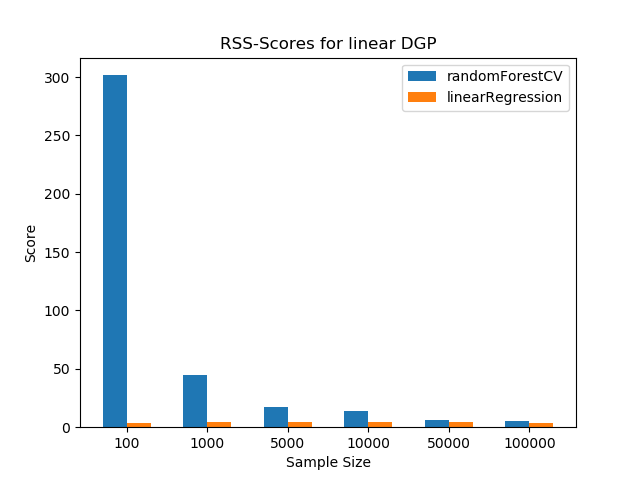
\includegraphics[width=120mm]{forest_vs_ols_linearDGP.png}}
    \caption
        {This plot illustrates the RSS for different training sample sizes for Random Forest and OLS.
        These samples where drawn from a linear DGP in accordance to equation (\ref{eq:linear_dgp}).
        The holdout set for calculating the RSS were drawn again for each training sample from the same DGP.
        It always contained 100 observations. In case of the Random Forest, for each sample the parameters
        got optimized again via cross validation.
        }
    \label{fig:forest_vs_ols_linearDGP}
\end{figure}

As one can see in figure \ref{fig:forest_vs_ols_linearDGP}, the RSS of the Random Forest converges
to that of the OLS for increasing sample sizes generated by the linear DGP. 

The non-linear DGP generates the data tuples \( (y, x_{1}, x_{2}) \) as follows:

\begin{equation}\label{eq:non_linear_dgp}
    y = \beta_{0} + \beta_{1} I(x_{1} >= 0, x_{2} >= 0) + \beta_{2} I(x_{1} >= 0, x_{2} < 0) + \beta_{3} I(x_{1} < 0) + \epsilon,
\end{equation}

whereas \( (\beta_{0}, \beta_{1}, \beta_{2}, \beta_{3}) \), \( x_{1}, x_{2} \) and \(  \epsilon \)
are the same as in the previous DGP.

\begin{figure}[H]
    \captionsetup{format=plain}
    \makebox[\textwidth]{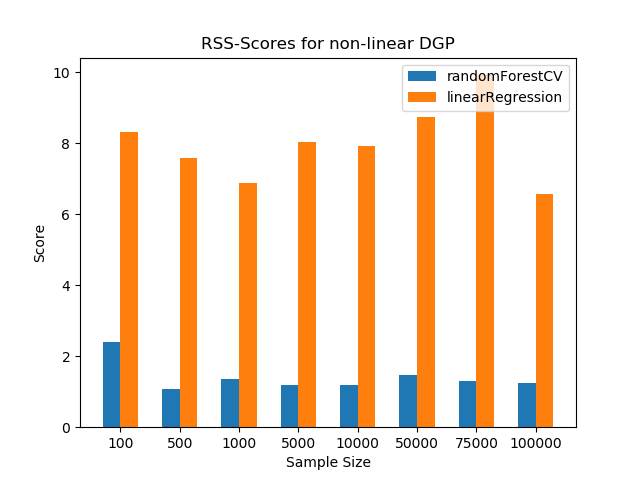
\includegraphics[width=120mm]{forest_vs_ols_nonlinearDGP.png}}
    \caption
        {This plot illustrates the RSS for different training sample sizes for Random Forest and OLS.
        These samples where drawn from a non-linear DGP in accordance to equation (\ref{eq:non_linear_dgp}).
        The holdout set for calculating the RSS were drawn again for each training sample from the same DGP.
        It always contained 100 observations. In case of the Random Forest, for each sample the parameters
        got optimized again via cross validation.
        }
    \label{fig:forest_vs_ols_nonLinearDGP}
\end{figure}

As one can see above in figure \ref{fig:forest_vs_ols_nonLinearDGP}, the Random Forest performs strictly better
than the OLS for any sample size. Due to this DGP resembling a stratification similar to
that of a Descision Tree, the RSS of the Random Forest converges relatively quickly while that of the OLS
remains unstable and high. 

	\subsection{Application of Random Forest on real data}
\label{sec:real_data}
As previously mentioned, we applied the Random Forest on the Titanic data set \cite{titanicData} to 
determine the survival of the passengers based on reported attributes like name title or booked cabin.
A major reason for choosing this data set was due to the fact that it consists of many categorical features.
In order to use the data to its fullest extent, we conducted additional feature engineering. 
Without that, many features remain unusable for our methods, 
because they contain missing values or values that are formatted as text.
Further, we split up the data set randomly into five folds via the K-fold method.
Then, the random forest got applied on each of the folds to obtain the classification rates.
Finally, we averaged these results to get a more representative performance evaluation of the Random Forest.
For the implementation of the feature engineering and the classification,
one can consult our code repository \cite{githubApplication}.
The Random Forest managed to achieve a total classification accuracy of 82.71\% on the holdout set.
According to the confusion matrix in figure \ref{fig:confusion_matrix_random_forest}, for passengers that died, 
the accuracy was slightly higher compared to those that survived. This is to be expected,
since deaths outnumber survivals considerably.

\begin{figure}[H]
    \captionsetup{format=plain}
    \makebox[\textwidth]{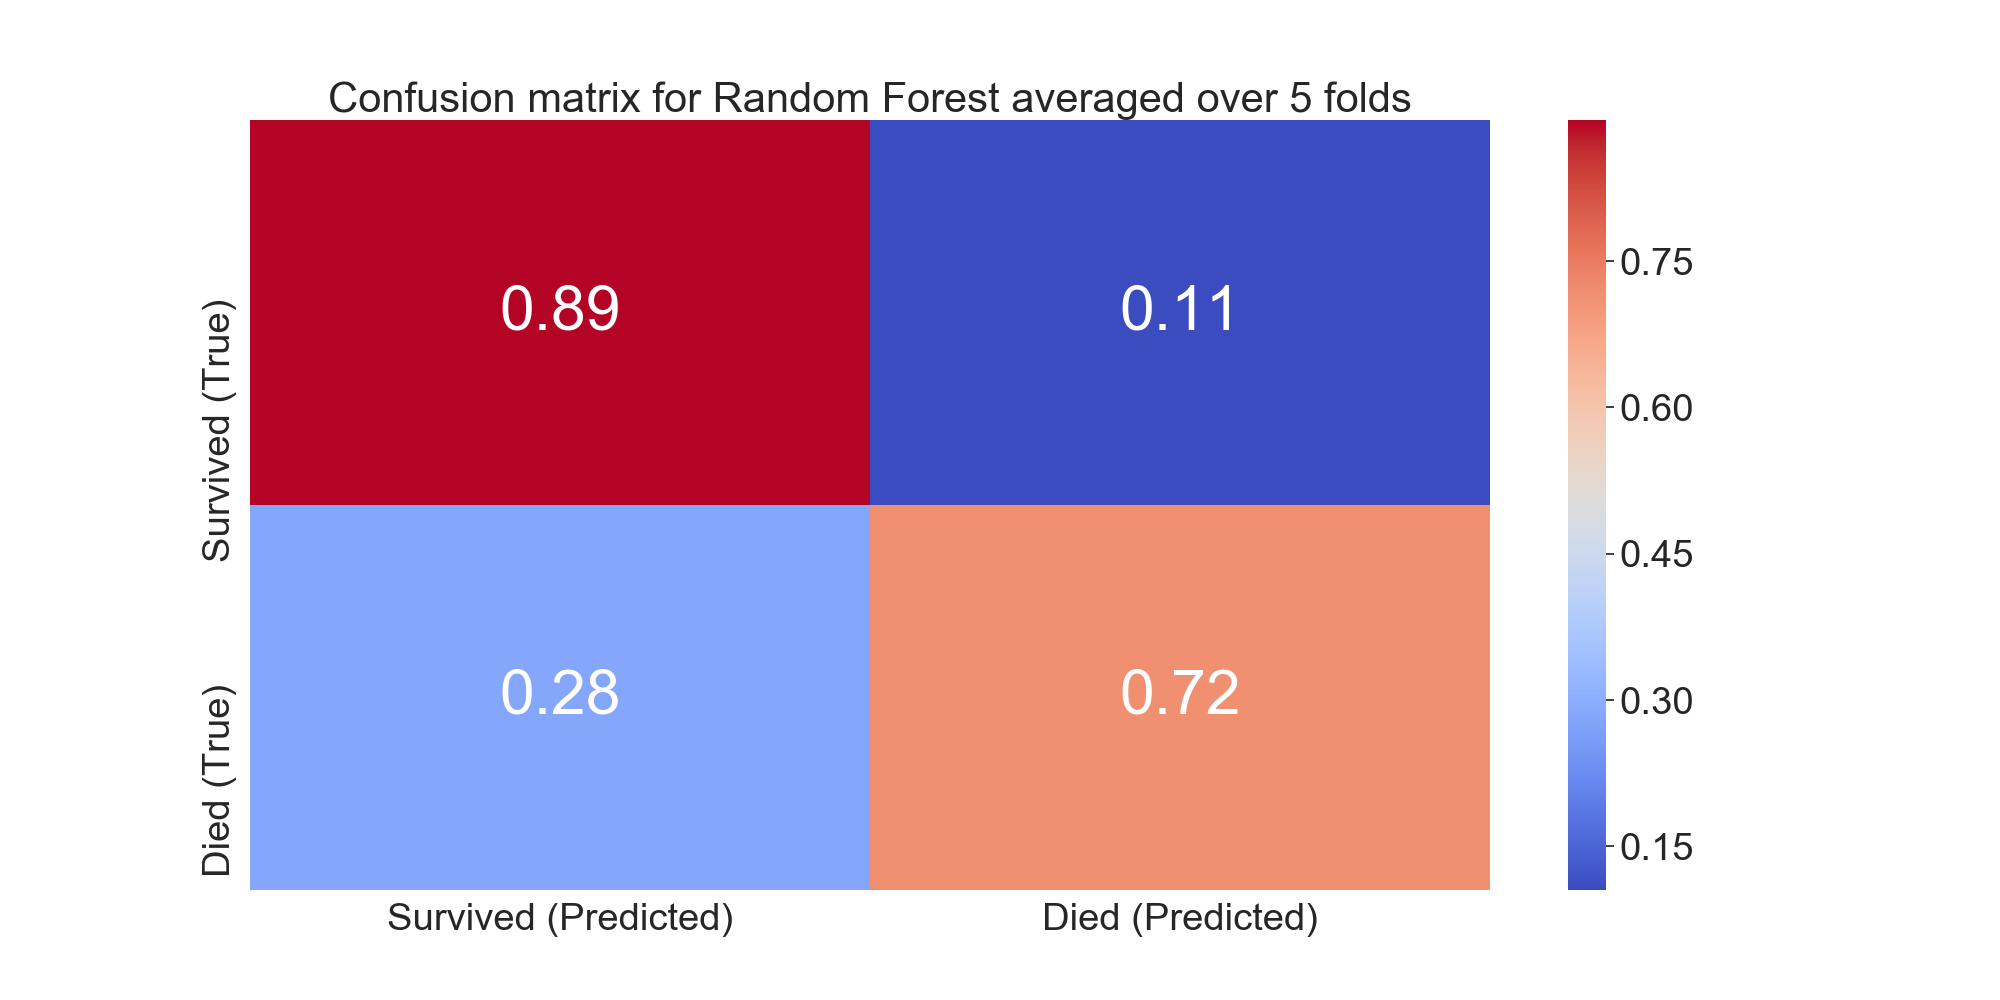
\includegraphics[width=200mm]{confusion_matrix_random_forest.png}}
    \caption
        {This plot illustrates the accuracy of the Random Forest's prediction on the Titanic data set.
        The data set got split into five folds on which the Random Forest got applied. 
        Then, the resulting combination of classification errors got averaged.
        The left axis indicates the true class membership, while the bottom one indicates the predicted one. 
        }
    \label{fig:confusion_matrix_random_forest}
\end{figure}


\section{Comparison to two boosting methods}
Before introducing AdaBoost and Gradient Boosting methods, 
it is essential to understand what boosting is. 
Like bagging, boosting is an approach which can be applied to many machine learning methods for 
classification or regression. Bagging uses bootstrap to create multiple datasets for training. 
In the next stage, bagging fits a separate Decision Tree to each training dataset, 
and then it combines all Decision Trees in order to create a single predictive model. 
Every Decision Tree is independent to others thanks to using bootstrap to create different training datasets. 
Boosting method works similarly, but in our case Decision Trees are grown sequentially. 
It means that each tree is built using information from previously built trees. 
Boosting does not involve bootstrap sampling. 
In this method, instead of bootstrap, each Decision Tree is fit on a modified version of 
the original dataset \cite{James2013}.

\subsection{AdaBoost Classifier}
\label{sec:adaboost}

\subsubsection{An introduction to the AdaBoost method}
Adaptive Boosting (Adaboost) was introduced by \cite{freund1997boosting} and we employ Adaboost as a comparison 
technique against Random Forest. In the Adaboost algorithm, instead of fully-grown trees as in Random Forest, 
we use trees with only one internal node and two leaves also called stumps. We consider those as weak-learners 
compared to trees since its depth and power are limited. Before generating stumps, 
we assign weights to observations in the sample. Normally the weight of each observation takes the value 
of $1/N$ as $N$ is the sample size. We generate a stump for each classifier in the data and compare them regarding 
their misclassification rate. After selecting the best classifier by using its stump's misclassification rate,
we compute its stump's significance. With that significance, we compute new weights for the sample. 
We repeat the algorithm sequentially for the sample with new weights until a stopping criterion is achieved. 
Generally, using the number of classifiers as the number of iteration is a common practice \cite{friedman2001elements}. 
After generating multiple stumps, we can predict an observation's class. 
We get the decision of every stump and form groups accordingly. 
Every outcome class has a group of stumps that predicts that class and every stump has its significance. 
After summing significance values of stumps in each group, the prediction is the class with the total highest significance. 
Although stumps are weak-learners, we exploit the error of a weak-learner to generate another weak-learner 
and iterating multiple times provides us with a powerful algorithm.

\subsubsection{Real Data Application of Adaboost}
The application of Adaboost is analogous to that of the Random Forest. 
That means that it got applied on the same five folds from the data set and its results got averaged.
When we employ Adaboost to predict the survival outcome of the passenger on Titanic, 
we achieve a mean classification rate of 82.94\% accuracy. By utilizing the confusion matrix of the classification 
and compare it with that of the Random Forest, we can see that for the non-survivals the result is almost the same,
but the Random Forest is slightly better when it comes to identifying survivors.

\begin{figure}[H]
    \captionsetup{format=plain}
    \makebox[\textwidth]{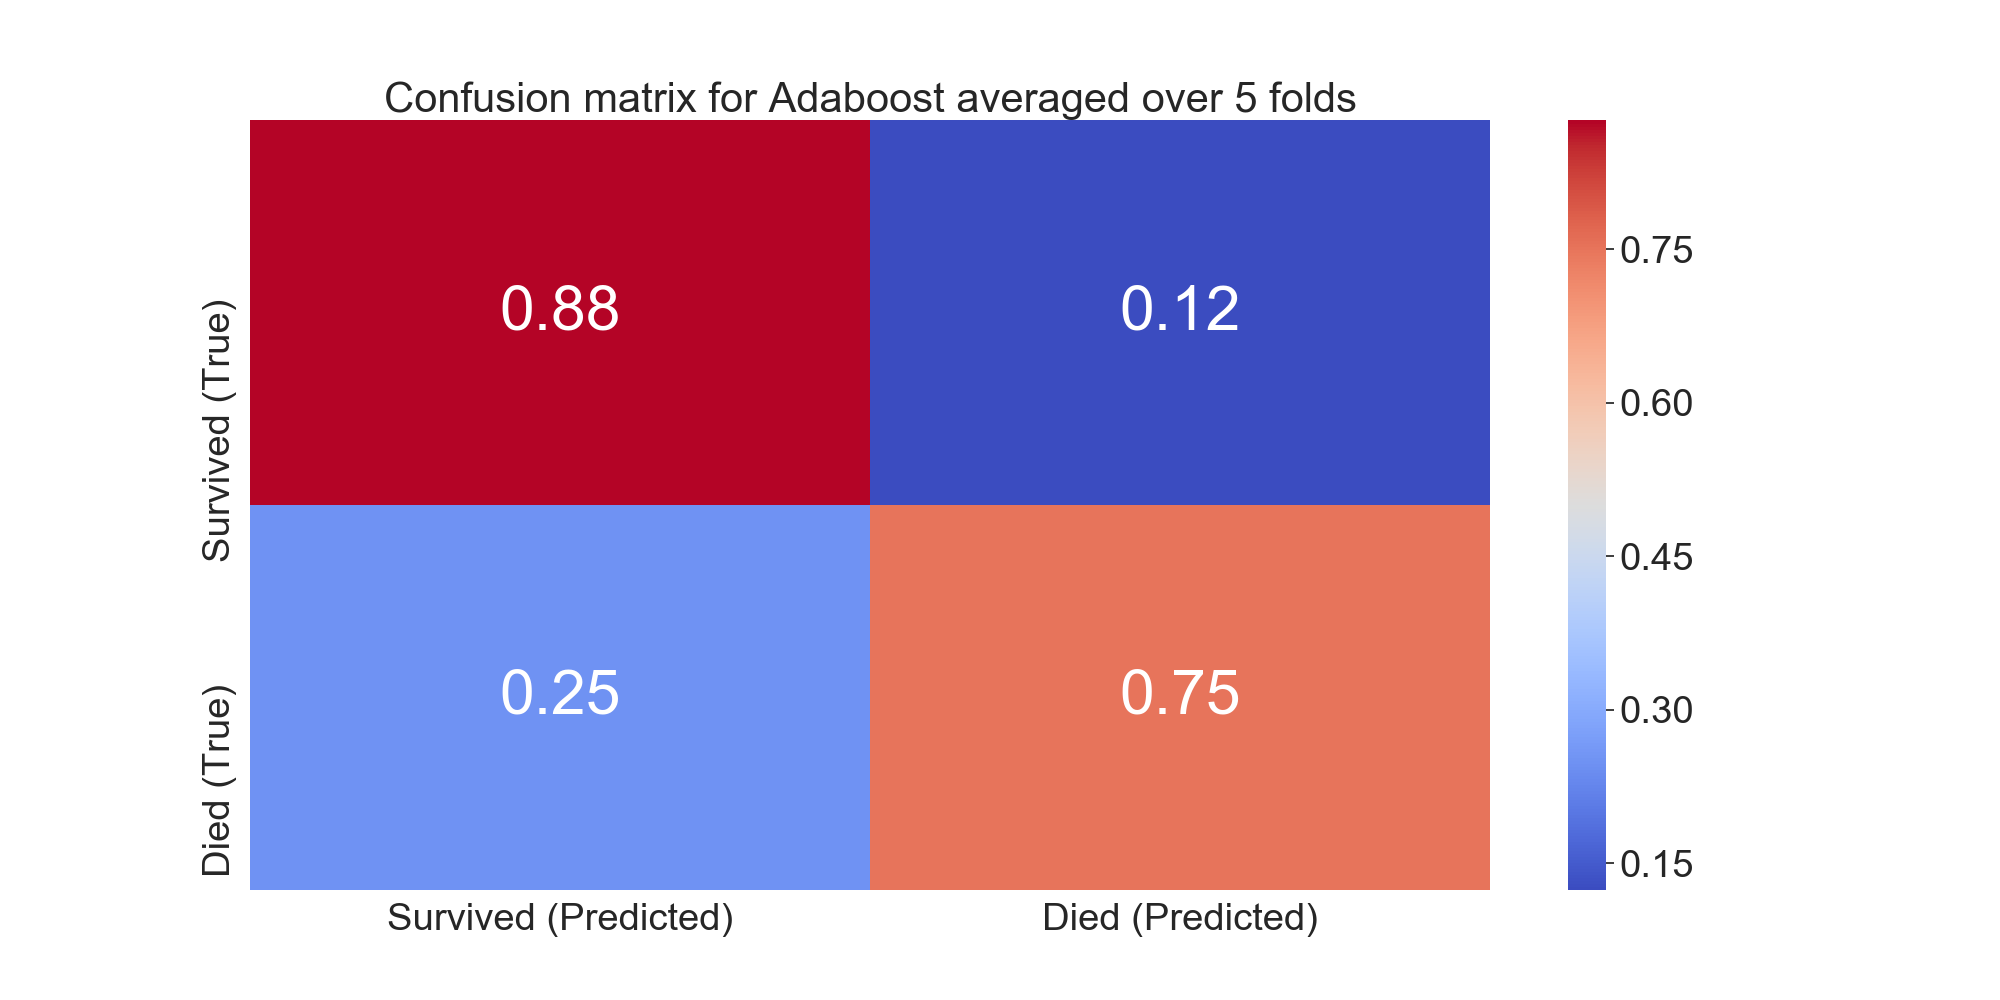
\includegraphics[width=200mm]{confusion_matrix_adaboost.png}}
    \caption
        {This plot illustrates the accuracy of the AdaBoost's prediction on the Titanic data set.
        The data set got split into five folds on which the Random Forest got applied. 
        Then, the resulting combination of classification errors got averaged.
        The left axis indicates the true class membership, while the bottom one indicates the predicted one.
        }
    \label{fig:confusion_matrix_adaboost}
\end{figure}


\subsection{Gradient Boosting Classifier}
\label{sec:gradient_boosting}

\subsubsection{An introduction to the Gradient Boosting method}
In Gradient Boosting the idea is to take a weak learning algorithm or hypothesis and make some corrections that will improve the power of this algorithm/hypothesis. In hypothesis boosting, we check every observation on which statistical learning method was trained on,
then you leave the observations which were correctly classified. Then the method creates a new weak learner and tests it only on the observations that were poorly classified. Next, the examples that were correctly classified are kept. The idea described above was used in the AdaBoost algorithm. In this algorithm, many weak learners are created by many Decision Trees that only have a single split. Created instances in the training dataset are weighted in the way that larger weights are assigned to instances that were difficult to classify. To the most difficult training instances, weaker learners are added sequentially. Gradient boosting classifiers are the Adaptive Boosting method, but it is combined with weighted minimization. After weighted minimization, all classifiers and weighted inputs are again calculated. The aim of gradient boosting classifiers is to minimize the loss and it operates in a similar way, like gradient descent in a neural network.

\subsubsection{Real data example}
The application of Gradient Boosting is analogous to that of the other methods. 
That means that it got applied on the same five folds from the data set and its results got averaged.
Thus, when we employ Gradient Boosting to predict the survival outcome of the passenger on Titanic, 
we achieve a mean classification rate of 82.15\% accuracy.

\begin{figure}[H]
    \captionsetup{format=plain}
    \makebox[\textwidth]{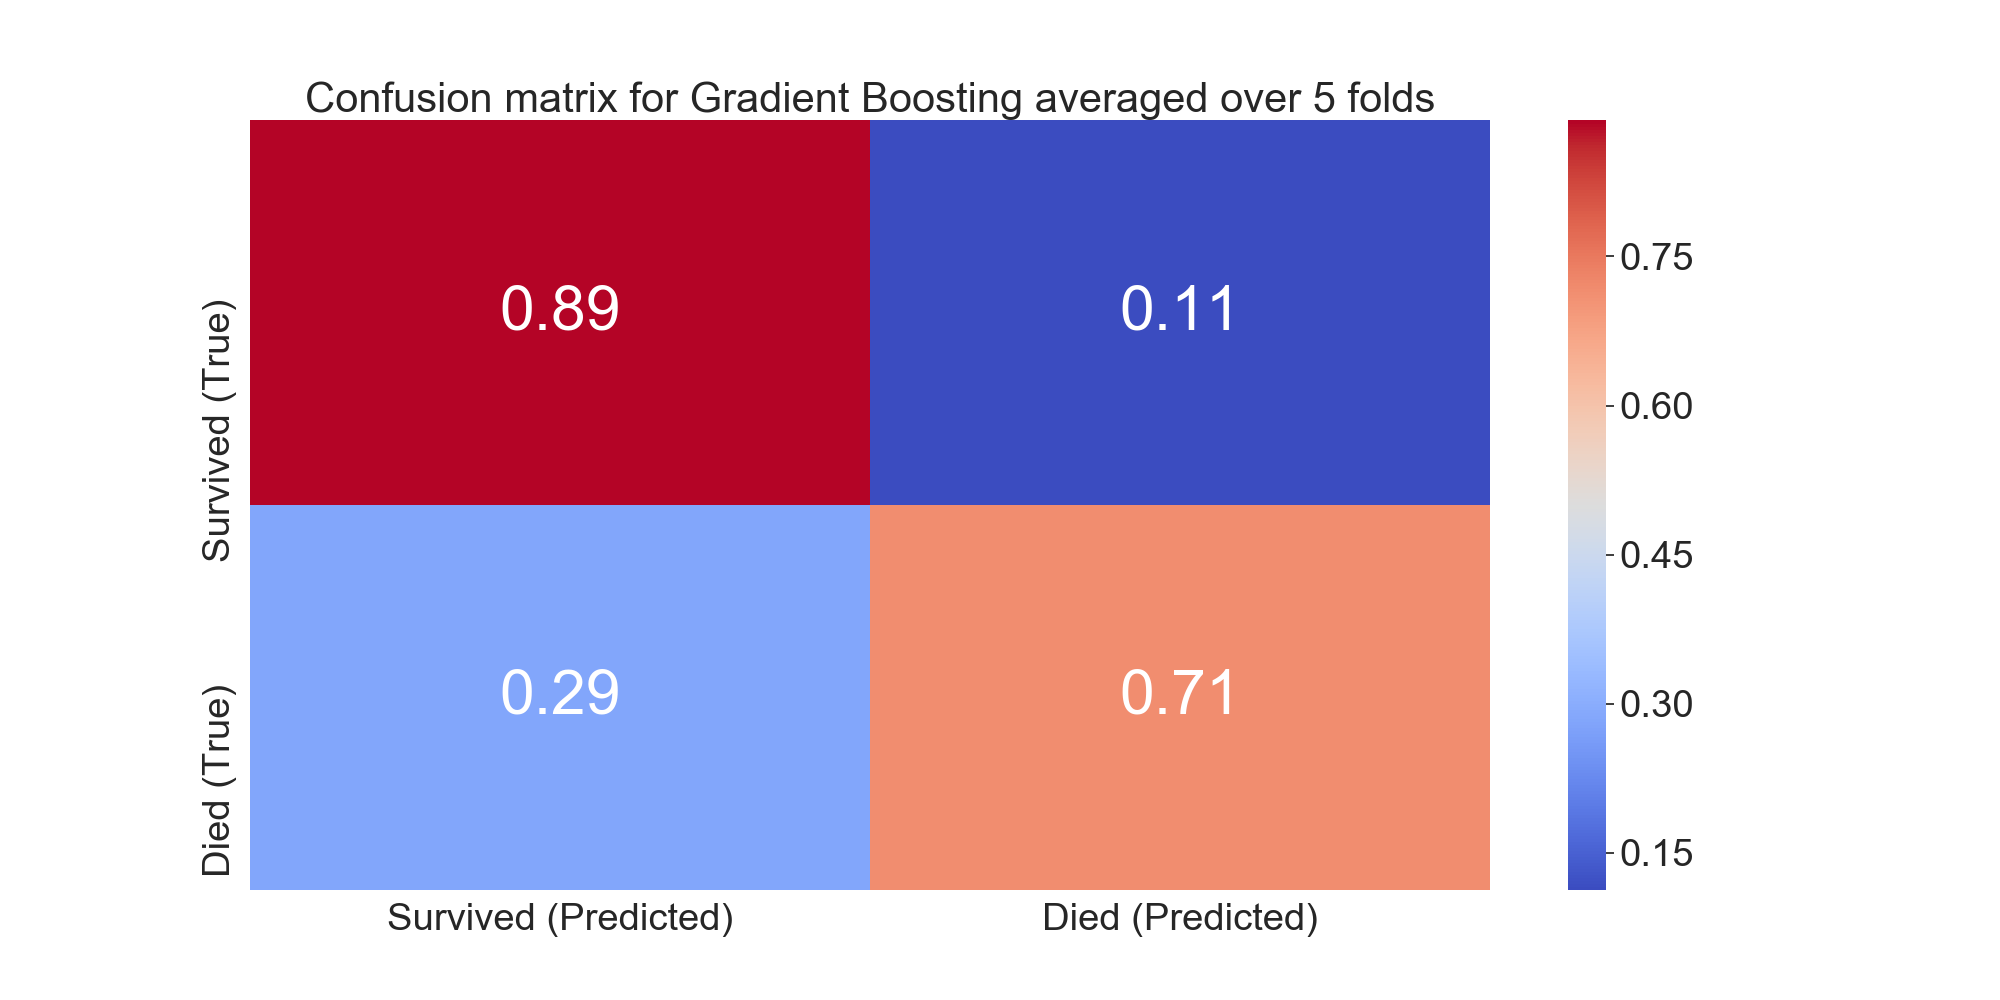
\includegraphics[width=200mm]{confusion_matrix_gradient_boosting.png}}
    \caption{This plot illustrates the accuracy of the Gradient Boosting's prediction on the Titanic data set.
    The data set got split into five folds on which the Random Forest got applied. 
    Then, the resulting combination of classification errors got averaged.
    The left axis indicates the true class membership, while the bottom one indicates the predicted one.}
    \label{fig:confusion_matrix_gradient_boosting}
\end{figure}



	\section{Conclusion and outlook}

We examined and applied one of the infamous machine learning algorithms, Random Forest. 
We started with explaining the Decision Trees and the room for improvement in it. 
As solutions of high-variance in Decision Trees, bagging, boosting and Random Forest are developed. 
Random Forest shows better predictions can be achieved with introducing randomness into the picture.
That randomness provides us with a decorrelated ensemble of trees and 
the increase in the number of trees yields lower error considering prediction purposes.
With using Random Forest, we are able to assess the importance of every variable and draw conclusions about data.
We explained the intuition of Random Forest in detail and included mathematical clarification. 
Finally, we applied Random Forest on both simulated and real data and compared with various methods. 
Considering results, Random Forest appears to be employed in the future as well, 
thus, a better understanding of the idea and the dynamics can give us a chance to improve. 
This paper aims to introduce the idea in detail and essentially a review and a showcase of the Random Forest algorithm. 
	% \newpage
	\section{Appendix}
\subsection{Bayes Model explanation}
\label{app:bayes_model}
We identified Bayes Model in equation (\ref{eq:bayes_model}) as such
\begin{align}
\phi_{\beta} & = \underset{c \,\in\, Y}{argmin} \; \mathbb{E}_{Y|X=x}\{L(Y,c) \} \notag\\
			 & = \underset{c \,\in\, Y}{argmin} \; P(Y \neq c \,| X = x) \notag\\
			 & = \underset{c \,\in\, Y}{argmax} \; P(Y = c \,| X = x)\notag
\end{align}

\subsection{Bias-variance decomposition of Squared Loss Function}
\label{app:bias_var_decomp}
We derived the result in equation (\ref{eq:decomp_squared_loss}) as follows;
\begin{align}
\boldsymbol{Err}(T_{D, \theta}(x)) & = \mathbb{E}_{Y|X=x}\{(Y-T_{D,\theta}(x))^2\} \notag \\
							  & = \mathbb{E}_{Y|X=x}\{(Y -\phi_{\beta}(x) +\phi_{\beta}(x) -T_{D,\theta}(x))^2\} \notag \\
							  & = \mathbb{E}_{Y|X=x}\{(Y-\phi_{\beta}(x))^2\} + \mathbb{E}_{Y|X=x}\{(\phi_{\beta}(x)-T_{D,\theta}(x))^2\} \notag \\
							  &	\: + \underbrace{\mathbb{E}_{Y|X=x}\{2(Y-\phi_{\beta}(x))(\phi_{\beta}(x)-T_{D,\theta}(x))\}}_\text{$=0$ \ since $ \mathbb{E}_{Y|X=x}(Y-\phi_{\beta}(x)) = 0$ from \ref{eq:bayes_eq_y}}  \notag \\
							  & = \underbrace{\mathbb{E}_{Y|X=x}\{(Y-\phi_{\beta}(x))^2\}}_\text{from \ref{eq:err_bayes} equals to $\boldsymbol{Err}(\phi_{\beta}(x))$} + \mathbb{E}_{Y|X=x}\{(\phi_{\beta}(x)-T_{D,\theta}(x))^2\}  \notag \\
							  & = \boldsymbol{Err}(\phi_{\beta}(x)) + (\phi_{\beta}(x)-T_{D,\theta}(x))^2\notag
\end{align}
We adopted following steps in the futher derivations of bias-variance decomposition in equation (\ref{eq:decomp_squared_loss_cont}).
\begin{align}
& \mathbb{E}_{D}\{(\phi_{\beta}(x) - T_{D,\theta}(x))^2 \} \notag \\
& = \mathbb{E}_{D}\{(\phi_{\beta}(x) - \mathbb{E}_{D}\{T_{D,\theta}(x)\} + \mathbb{E}_{D}\{T_{D,\theta}(x)\} - T_{D,\theta}(x))^2\} \notag \\
& = \mathbb{E}_{D}\{(\phi_{\beta}(x) - \mathbb{E}_{D}\{T_{D,\theta}(x))^2\} 
	+ \mathbb{E}_{D}\{(\mathbb{E}_{D}\{T_{D,\theta}(x)\} - T_{D,\theta}(x))^2\} \notag \\
&\: \: + \mathbb{E}_{D}\{2(\phi_{\beta}(x) - \mathbb{E}_{D}\{T_{D,\theta}(x)\})(\mathbb{E}_{D}\{T_{D,\theta}(x)\} - T_{D,\theta}(x))\} \notag \\
& \text{since $\mathbb{E}_{D}\{\mathbb{E}_{D}\{T_{D,\theta}(x)\} - T_{D,\theta}(x)\} = \mathbb{E}_{D}\{T_{D,\theta}(x)\} - \mathbb{E}_{D}\{T_{D,\theta}(x)\} = 0$} \notag \\
& = \mathbb{E}_{D}\{(\phi_{\beta}(x) - \mathbb{E}_{D}\{T_{D,\theta}(x))^2\} 
	+ \mathbb{E}_{D}\{(\mathbb{E}_{D}\{T_{D,\theta}(x)\} - T_{D,\theta}(x))^2\} \notag \\
& = (\phi_{\beta}(x) - \mathbb{E}_{D}\{T_{D,\theta}(x))^2 + \mathbb{E}_{D}\{(\mathbb{E}_{D}\{T_{D,\theta}(x)\} - T_{D,\theta}(x))^2\}\notag
\end{align}

\subsection{Kohavi's decomposition of zero-one loss function}
\label{app:kohavi_decomp}
Kohavi proposed an alternative decomposition for zero-function \cite{kohavi1996bias}. 
Our notation differs in some extent from Kohavi's paper to be coherent with out prior findings. 
The zero-one loss function is defined as
\begin{align}
L(\phi_{\beta}(x), T_{D,\theta}(x)) = 1 - \delta(\phi_{\beta}(x), T_{D, \theta}(x)) \notag
\end{align}
where $\delta(\phi_{\beta}(x), T_{D, \theta}(x)) = 1$ if $\phi_{\beta}(x) = T_{D, \theta}(x)$ and 0 otherwise. The generalization error (misclassification rate in the paper) is defined and extented as
\begin{align}\label{eq:kohavi_eq}
\boldsymbol{Err}(T_{D, \theta}(x)) 
& = L(\phi_{\beta}(x), T_{D,\theta}(x) P(\phi_{\beta}(x), T_{D, \theta}(x)) \notag \\
& = \sum_{\phi_{\beta}(x), T_{D, \theta}(x)} [1 - \delta(\phi_{\beta}(x), T_{D, \theta}(x))] P(\phi_{\beta}(x), T_{D, \theta}(x)) \notag \\
& = 1 - \sum_{y \in Y} P(\phi_{\beta}(x) = T_{D, \theta}(x)) = y)
\end{align}
Even if in the Kohavi's paper it is stated that the last step is a 
simplified version of the extended Bayesian Formalism \cite{wolpert2018relationship}, 
there is not enough explanation to explicitly show the mathematical derivation nor the intuition. If we continue examine the equation (\ref{eq:kohavi_eq}) we get the following decomposition;
\begin{align}\label{eq:kohavi_eq1}
\boldsymbol{Err}(T_{D, \theta}(x))
& = 1 - \sum_{y \in Y} P(\phi_{\beta}(x) = T_{D, \theta}(x)) = y) \notag\\
& = \sum_{y \in Y} -P(\phi_{\beta}(x) = T_{D, \theta}(x)) = y) + \sum_{y \in Y} P(\phi_{\beta}(x) = y) P(T_{D, \theta}(x)) = y) \notag\\
& + \sum_{y \in Y}[-P(\phi_{\beta}(x) = y) P(T_{D, \theta}(x)) = y) + \dfrac{1}{2}P(T_{D, \theta}(x) = y)^2 + \dfrac{1}{2}P(\phi_{\beta} = y)^2] \notag\\
& + [\dfrac{1}{2} - \dfrac{1}{2}\sum_{y \in Y} P(T_{D,\theta}(x)= y)^2] + [\dfrac{1}{2} - \dfrac{1}{2}\sum_{y \in Y} P(\phi_{\beta}(x)= y)^2]
\end{align}
Rearranging equation (\ref{eq:kohavi_eq1}) yields
\begin{align}\label{eq:kohavi_eq2}
\boldsymbol{Err}(T_{D, \theta}(x))
& = \sum_{y \in Y} [P(T_{D,\theta}(x)=y)P(\phi_{\beta}(x) = y) - P(T_{D,\theta}(x) = \phi_{\beta}(x) = y)]\tag{$*$} \\
& + \dfrac{1}{2}\sum_{y \in Y} [P(T_{D,\theta}(x)=y) - P(\phi_{\beta}(x) = y)]^2\notag \\
& + \dfrac{1}{2}(1 - \sum_{y \in Y}P(T_{D, \theta}(x) = y)^2) + \dfrac{1}{2}(1 - \sum_{y \in Y}P(\phi_{\beta}(x) = y)^2)\notag \\
\end{align}
The $*$ term is the covariance between Bayes Model and Decision Tree which equals to zero since by construction Bayes Model cannot be dependent of any model. Then the decomposition becomes;
\begin{align}
\boldsymbol{Err}(T_{D, \theta}(x)) = \sum_{x} P(x)(\boldsymbol{Err}(\phi_{\beta}) + bias^2 + variance) \notag
\end{align}
where
\begin{align}
\boldsymbol{Err}(\phi_{\beta}) & = \dfrac{1}{2}(1 - \sum_{y \in Y}P(\phi_{\beta}(x) = y)^2)\tag{Bayes Error} \\
bias^2 & = \dfrac{1}{2}\sum_{y \in Y} [P(T_{D,\theta}(x)=y) - P(\phi_{\beta}(x) = y)]^2\notag \\
variance & = \dfrac{1}{2}(1 - \sum_{y \in Y}P(T_{D, \theta}(x) = y)^2) \notag
\end{align}
Since the outcome of Kohavi's decomposition is not as explanatory as our prior findings and without assuming a certain type of distribution for the sample \cite{louppe2014understanding}, we wanted to explain mathematical dynamics of random forest with using the squared loss function alongside zero-one loss function.

\subsection{Correlation Coefficient}
\label{app:corr_coef}
Using the definition of the Pearson's correlation coefficient and the property of $\theta'$ and $\theta''$ following the same distribution, we derived correlation coefficient as such
\begin{align}
\rho(x) & = \dfrac{\mathbb{E}_{D,\theta',\theta''}\{(T_{D,\theta'}(x) - \mu_{D,\theta'}(x))(T_{D,\theta''}(x) - \mu_{D,\theta''}(x))\} }				{\sigma_{D,\theta'}(x)\sigma_{D,\theta'}(x)}\notag \\
		& = \dfrac{\mathbb{E}_{D,\theta',\theta''}\{T_{D,\theta'}(x)T_{D,\theta''}(x) - T_{D,\theta'}(x)\mu_{D,\theta''}(x) - T_{D,								\theta''}(x)\mu_{D,\theta'}(x) + \mu_{D,\theta'}(x)\mu_{D,\theta''}(x))\} }
				{\sigma_{D,\theta}^2(x)} \notag \\
		& = \dfrac{\mathbb{E}_{D,\theta',\theta''}\{T_{D,\theta'}(x) T_{D,\theta''}(x)\} - \mu_{D,\theta}^2(x)}{\sigma_{D,\theta}^2(x)}\notag
\end{align}

With an alternative decomposition, we can state that $\rho(x)$ is non-negative 
\cite{louppe2014understanding} \cite{geurts2002contributions}. 
Being that said the findings we explored with decomposing the variance of the squared loss function are robust.

\subsection{Decomposition of Variance}
\label{app:var_decomp}
The derivation of equation (\ref{eq:decomp_var}) is as follows;

\begin{align}
\mathbb{V}\{\boldsymbol{RF}\} & = \mathbb{V}_{D, \theta_{1}, \theta_{2},..., \theta_{B}}\{\boldsymbol{RF}_{D, \theta_{1},\theta_{2},..., \theta_{B}}(x) \}\notag \\
& = \mathbb{V}_{D, \theta_{1}, \theta_{2},..., \theta_{B}}\{\dfrac{1}{B}\sum_{b=1}^{B} T_{D,\theta_{b}}(x)\} \notag
\end{align}
Using $\mathbb{V}\{aX\} = a^2\mathbb{V}\{X\} = a^2 (\mathbb{E}\{X^2\} - \mathbb{E}\{X\}^2$, variance of random forest equals to

\begin{align}
\mathbb{V}\{\boldsymbol{RF}\} = \dfrac{1}{B}\left[\mathbb{E}_{D, \theta_{1}, \theta_{2},..., \theta_{B}}\{( \sum_{b=1}^{B} T_{D, \theta_{b}}(x))^2 \} - \mathbb{E}_{D, \theta_{1}, \theta_{2},..., \theta_{B}}\{( \sum_{b=1}^{B} T_{D, \theta_{b}}(x)) \}^2\right] \notag
\end{align}

Following Louppe's derivations, we can rewrite the variance as pairwise products of any two trees using parameters $\theta_{i}$ and $\theta_{j}$;

\begin{align}
\mathbb{V}\{\boldsymbol{RF}\} & = \dfrac{1}{B}[\mathbb{E}_{D, \theta_{1}, \theta_{2},..., \theta_{B}}\{\sum_{i,j} T_{D,\theta_{i}}(x) T_{D,\theta_{j}}(x)\} - (B \mu_{D,\theta}(x))^2] \notag
\end{align}
where $\mu_{D, \theta}$ is the average prediction of all ensembled trees and derived in equation (\ref{eq:mu}).
\begin{align}
\mathbb{V}\{\boldsymbol{RF}\} & = \dfrac{1}{B^2}\left[\sum_{i,j} \mathbb{E}_{D, \theta_{i}, \theta_{j}}\{T_{D,\theta_{i}}(x) T_{D,\theta_{i}}(x)\} - B^2 \mu_{D,\theta}^2(x)\right]\notag \\
& = \dfrac{1}{B^2}\left[B\mathbb{E}_{D,\theta}\{T_{D,\theta}(x)^2\} + (B^2 - B) \mathbb{E}_{D, \theta_{i}, \theta_{j}}\{T_{D,\theta_{i}}(x) T_{D,\theta_{i}}(x)\} - B^2 \mu_{D,\theta}^2(x)\right]\notag \\
& = \dfrac{1}{B^2}\left[B(\sigma_{D,\theta}^2(x) + \mu_{D,\theta}^2(x)) + (B^2 - B) (\rho(x)\sigma_{D,\theta}^2(x) + \mu_{D, \theta}^2(x)) - B^2 \mu_{D,\theta}^2(x)\right] \notag \\
& = \dfrac{\sigma_{D,\theta}^2(x)}{B} + \rho(x)\sigma_{D,\theta}^2(x) - \rho(x)\dfrac{\sigma_{D,\theta}^2(x)}{B}\notag \\
& = \rho(x)\sigma_{D,\theta}^2(x) + \dfrac{1 - \rho(x)}{B}\sigma_{D,\theta}^2(x) \notag
\end{align}
\subsection{Bias-Variance Decomposition Figures}
\begin{figure}[H]
	\centering
	\captionsetup{format=plain}
	\makebox{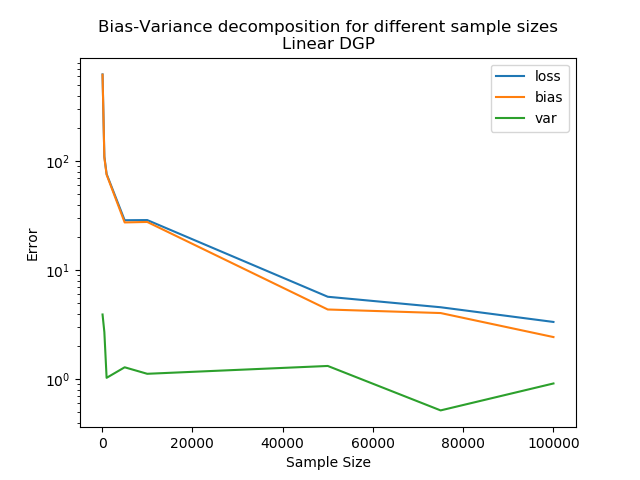
\includegraphics[width=120mm]{bias_var_linearDGP.png}}
	\caption{This figure demonstrates the decomposition of the expected generalization error in linear DGP. 
			The expected generalization error is denoted with loss. 
			As sample size increases both the expected generalization error and bias tend to decrease. 
			Although the variance does not follow a pattern, in theory, we expect low variance and 
			variance remains to be low for all sample sizes.}
	\label{fig:bias_var_linear}
\end{figure}

\begin{figure}[H]
	\centering
	\captionsetup{format=plain}
	\makebox{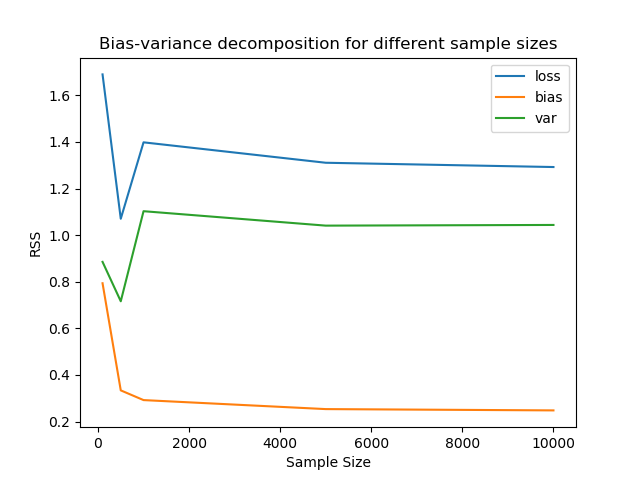
\includegraphics[width=120mm]{bias_var_nonlinearDGP.png}}
	\caption{This figure demonstrates the decomposition of the expected generalization error in nonlinear DGP. 
			The expected generalization error is denoted with loss. 
			The expected generalization error is driven primarily 
			by variance and bias remains to be low for all sample sizes. 
			As expected, Random Forest decreases the variance and bias remains to be low due to low biasness of Decision Tree estimates.}
	\label{fig:bias_var_nonlinear}
\end{figure}





	% \pagebreak

	\printbibliography

	% \section{Declaration}
	% I hereby certify that this material is my own work, that I used only those sources and resources referred to in the thesis, and that I have identified citations as such.
			
	% \vspace{0.3in}

	% \noindent Bonn, \today

\end{document}
